Para servir de punto de comparaci\'on, en este trabajo tambi\'en analizaremos el 
comportamiento de arquitecturas como NVIDIA CUDA e Intel Xeon Phi con respecto a procesadores
CPU Estandar. En particular nos enfocaremos en la arquitectura Intel x86 de 64 bits.

Si bien las dem\'as arquitecturas analizadas difieren fuertemente de x86-64, estas diferencias
surgen de tendencias relativamente recientes en el desarrollo de procesadores que llevan a
tomar decisiones de \textit{tradeoffs} similares tambi\'en en procesadores m\'as usuales.

Una de estas tendencias es la disminuci\'on en el crecimiento de la \textit{performance} de
cada procesador o \textit{core} con respecto a a\~nos anteriores, empezando aproximadamente
desde 2003~\cite{HennessyPatterson}.

\begin{figure}[htbp]
    \centering
    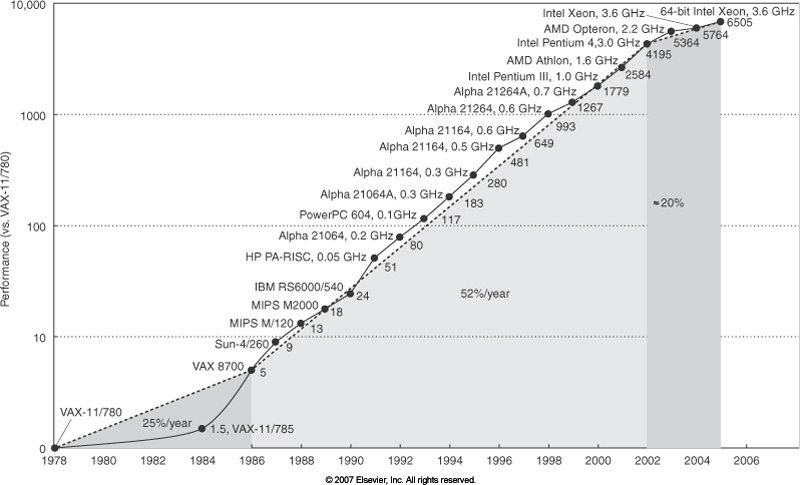
\includegraphics[width=\textwidth]{images/processor-performance.jpg}
    \caption{Performance de procesador en los \textit{benchmarks} SPEC on respecto a VAX-11/780. Tomado de~\cite{HennessyPatterson}}
    \label{processor_performance}
\end{figure}

Las razones de esto son diversas, incluyendo limites f\'isicos de cantidad de transistores
por \textit{chip} por disipaci\'on de calor, pero tambi\'en involucran otros factores 
relacionados con los tipos de \textit{paralelismo} empleados.

A grandes rasgos, existen los siguientes tipos de paralelismo que puede aprovechar una
arquitectura para mejorar la \textit{performance} de ejecuci\'on:

\begin{itemize}
    \item \textit{Instruction Level Parallelism}: Este tipo de optimizaciones, que buscan
    ejecutar la mayor cantidad de instrucciones en un mismo hilo de ejecuci\'on simultaneamente,
    eran las m\'as usuales en los monoprocesadores. Optimizaciones de este estilo incluyen
    \textit{pipelines} de procesador para ejecutar multiples instrucciones de manera solapada,
    ejecuci\'on superescalar fuera de \'orden para ejecutar multiples instrucciones que 
    utilizan unidades del procesador distintas o que no dependen una de la otra, ejecuci\'on
    especulativa (basada en predicci\'on de saltos del procesador), etc. 

    \item \textit{Data Level Parallelism}: Consideran las optimizaciones cuyo prop\'osito es
    lograr aplicar una misma operaci\'on a cada elemento de un conjunto datos simultaneamente 
    en un mismo hilo de ejecuci\'on. Concierte por ejemplo a operaciones de vectorizaci\'on, 
    presentes en procesadores de la familia Intel mediante el set de operaciones SSE 
    (Streaming SIMD Extensions) o AVX (Advanced Vector eXtensions), que incluyen instrucciones
    para actuar sobre varios enteros o valores de punto flotante (por ejemplo, sumarlos, etc.)
    que estan puestos en un arreglo, al mismo tiempo. Por eso este modelo se denomina SIMD
    (Single Instruction, Multiple Data).

    \item \textit{Thread Level Parallelism}: Alejandonos de los procesadores monocore, tenemos
    la aparici\'on de m\'aquinas con m\'as de un procesador, que permiten por lo tanto hilos
    de ejecuci\'on totalmente independientes. Estos procesadores usualmente
    comparten la memoria principal (arquitectura SMP, \textit{Symmetric Multiprocessing}), lo
    cual conlleva a esfuerzo adicional para mantener consistencia y coherencia de la misma, y
    que no se convierta en un cuello de botella.  Adem\'as, existen optimizaciones por 
    \textit{hardware} para lograr multiples hilos de ejecuci\'on en un mismo procesador
    (por ejemplo Intel Hyperthreading).
\end{itemize}

La primera de estas maneras de explotar paralelismo fue la que prevaleci\'o mucho tiempo los
procesadores dominantes en el mercado (a pesar de que la taxonom\'ia de Flynn~\cite{HennessyPatterson} ya incluye 
procesadores que explotan todas ellas). La segunda y la tercera, base de arquitecturas como NVIDIA CUDA y Xeon Phi, 
est\'an tambi\'en haciendo aparici\'on en procesadores basados en x86: El procesador Intel Xeon E7-8800 posee 10 \textit{cores}
(2 hilos de ejecuci\'on por \textit{core}) a 2.4 GHz con un set de instrucciones SSE 4.2 que permite ejecutar una misma instrucci\'on
sobre 4 valores de punto flotante IEEE-754 de 32 bits (usando registros SSE de 128 bits)~\cite{XeonE78800Spec}. 

Estas tendencias en la busqueda de lograr m\'as hilos de ejecuci\'on y m\'as procesamiento simult\'aneo de datos, adem\'as
de mejoras al nivel instrucci\'on, tiene un impacto fuerte que diferencia sistemas pensados para computo intensivo de
sistemas de prop\'osito general. Este cambio de modelo requiere m\'as esfuerzo por parte del programador para aprovecharlo
correctamente, lo cual tambi\'en genera inter\'es en herramientas y literatura que sirva de gu\'ia al desarrollador, que
ahora no puede simplemente esperar a que la performance de un procesador se duplique cada 18 meses, y debe estructurar su
c\'odigo para hacer uso de los nuevos recursos que dispone.
